
% Document type and layout
\documentclass[parskip=half, titlepage=yes, 12pt, BCOR=12mm, DIV=calc]{scrartcl}

% Praeambel = definition of layout and packages
%!TeX root=Main.tex


%%%%%%%%%%%%%%%%%%%%%%%%%%%%%%%%%%%%%%%%%%%%%%%%%%%
%%%           Allgemeine Einstellungen          %%%
%%%%%%%%%%%%%%%%%%%%%%%%%%%%%%%%%%%%%%%%%%%%%%%%%%%


% Pakete für die Darstellung und Eingabemöglichkeit von Umlauten
\usepackage[T1]{fontenc}
\usepackage[utf8]{inputenc}


% Schriftarten anpassen auf helvet für seriefenlose Schrift 
% und passende Mathematik-Schrift
\usepackage{mathptmx}
\usepackage{courier}
\usepackage{microtype}     % Paket für Randausgleich

% Paket zum verwendeten erweiterter Floatoptionen
\usepackage{float}

% Pakete zum Einbinden von Bildern und Farben
\usepackage{xcolor}
\usepackage{graphicx}           


% Verwendung englischer Begriffe für automatisch generierte Worte
% wie z.B. "Contents" anstelle von "Inhaltsverzeichnis"
\usepackage[english]{babel}

% Paket um Dummy-Text/Blindtext zu erzeugen
\usepackage{blindtext}


% Mathematik Befehle und Formelsätze
\usepackage{amsmath} 
\usepackage{amssymb}
\usepackage{amsthm}
\usepackage[free-standing-units,locale = DE]{siunitx} % SI-Einheiten
\usepackage[english]{algorithm2e}     % Algorithmen
%\usepackage{MnSymbol}                % große Klammern -> falsch benutzt


% Tabellen
\usepackage{booktabs}     % Schöne Tabellen
\usepackage{supertabular} % Tabellen über mehr als eine Seite

%%%%% Literaturverzeichnis


% Literaturverzeichnis mitt BibLaTeX und Biber erstellen
\usepackage[style=numeric, sorting=none, backend=biber]{biblatex}
\addbibresource{Literature.bib}



%%%%%%%%%%%%%%%%%%%%%%%%%%%%%%%%%%%%%%%%%%%%%%%%%%%
%%%            Dokumentenlayout                 %%%
%%%%%%%%%%%%%%%%%%%%%%%%%%%%%%%%%%%%%%%%%%%%%%%%%%%


% Eigene Style-Klasse fuer eigenes Titelblatt
\usepackage{Titel}


% Allgemeine Papiergometrie
\usepackage{geometry}
\geometry{a4paper}


% Abstand der weißen Ränder
\geometry{margin=3.0cm, inner=2.5cm, outer=2.5cm} 


% Zeilenabstand auf 1,5 setzen
\usepackage[onehalfspacing]{setspace}
    \AfterTOCHead{\singlespacing}
% KOMA Klasse für europ. Layout - Wird hier nicht verwendet
  %  \KOMAoptions{DIV=last}     


% Zeit und Datumsbefehle  
\usepackage{scrdate, scrtime}   


% Erweitere Layout-Optionen
\usepackage{scrlayer-scrpage}   


% Zusätzliches Seitenlayout selbst definieren
\pagestyle{scrheadings}         


%%%%% Kopf- und Fußzeile

% Belegung von KOMA Variablen für Kopf- und Fußzeilen Gestaltung
\newcommand{\footlinetext}{\footnotesize \textsf{\color{gray}  Martin Michel, B-AMP 6  \normalsize}}

\KOMAoptions{headsepline = no, footsepline = yes}
\ihead{\headmark}
\chead{}
\ohead{}
\ifoot{\footlinetext}
\cfoot{\color{gray}\pagemark}
\ofoot{\footnotesize \textsf{\color{gray}  Radio frequency ablation with finite elements \normalsize}}



%%%%%%%%%%%%%%%%%%%%%%%%%%%%%%%%%%%%%%%%%%%%%%%%%%%
%%%   Einstellungen für Programmierquellcode    %%%
%%%%%%%%%%%%%%%%%%%%%%%%%%%%%%%%%%%%%%%%%%%%%%%%%%%


% Paket und Spezifikation der Parameter zur Darstellung 
% von Programmcode mit Courier-Schriftart
\usepackage{listings}  % Darstellung von Quellcode
\usepackage{courier}   % Schriftart laden


% Anzeigeeinstellungen für C++ Code
% Siehe Dokumentation für weitere Sprachen
\lstset{
    language=C++,
    basicstyle=\footnotesize\ttfamily,  % Standardschrift
    numbers=left,                       % Ort der Zeilennummern
    numberstyle=\tiny,                  % Stil der Zeilennummern
    %stepnumber=2,  % Abstand zwischen den Zeilennummern
    numbersep=5pt,  % Abstand der Nummern zum Text
    tabsize=2,      % Groesse von Tabs
    extendedchars=true, %
    breaklines=true,    % Zeilen werden Umgebrochen
    keywordstyle=\color{blue}\bfseries,
    frame=b,
    % keywordstyle=[1]\textbf, % Stil der Keywords
    % keywordstyle=[2]\textbf, %
    % keywordstyle=[3]\textbf, %
    % keywordstyle=[4]\textbf, \sqrt{\sqrt{}} %
    stringstyle=\color{magenta}\ttfamily, % Farbe der Strings
    showspaces=false,   % Keine Leerzeichen anzeigen 
    showtabs=false,     % Keine Tabs anzeigen 
    % xleftmargin=17pt,  % Abstände
    % framexleftmargin=17pt,
    % framexrightmargin=5pt,
    % framexbottommargin=4pt,
    commentstyle=\color{green!100!blue}\bfseries,
    %backgroundcolor=\color{grey},
    showstringspaces=true,      % Leerzeichen in Strings anzeigen
    morekeywords={__global__},  % additional language specific keywords
    morecomment=[l]
    }

    
% Syntax-Highligthing aktivieren
\lstloadlanguages{ 
    %[Visual]Basic
    %Pascal
    C,
    C++,
    %XML
    %HTML
    Matlab
    %Java
}



%%%%%%%%%%%%%%%%%%%%%%%%%%%%%%%%%%%%%%%%%%%%%%%%%%%
%%%           Layout im PDF Viewer              %%%
%%%    Muss als letztes Paket geladen werden    %%%
%%%%%%%%%%%%%%%%%%%%%%%%%%%%%%%%%%%%%%%%%%%%%%%%%%%


\usepackage{hyperref}           
\hypersetup{
    plainpages=false,
    linktocpage=true,
    breaklinks=true,
    colorlinks=true,
    linkcolor=black,%blue,
    anchorcolor=black,
    citecolor=black,%green,
    filecolor=black,%blue,
    urlcolor=black,%blue%
    pdfstartview={FitV},
    pdfview={FitH},
    pdfpagelayout={SinglePage},
    pdfpagemode={None},
}




%%%%%%%%%%%%%%%%%%%%%%%%%%%%%%%%%%%%%%%%%%%%%%%%%%%
%%%          Variablen zum Belegen              %%%
%%%%%%%%%%%%%%%%%%%%%%%%%%%%%%%%%%%%%%%%%%%%%%%%%%%


%%%%%% Variablen für Titelblatt

\DAAutor{Martin Michel}
\DATyp{Report of the application project}
\DAAutorAdresse{Keßlerplatz 12\par DE-90489 Nuremberg}
\DAFachbereich{AMP}
\DATitel{Simulation of a medical therapy \\ method with finite elements}
\DABetreuerA{Prof.\ Dr.\ rer.\ nat.\ Tim\ Kröger}
\DABetreuerB{Prof.\ Dr.\ rer.\ nat.\ habil.\ Jörg\ Steinbach}
\DABetreuerC{Prof.\ Dr.\ rer.\ nat.\ Thomas\ Lauterbach}
\DAOrt{Nuremberg}
\DAAbgabedatum{31.\,August\,2020}


\usepackage{amsthm}
\usepackage{lipsum}

%% Actual document
\begin{document}


% Title and registers
\maketitle
\tableofcontents

\clearpage

% \listoffigures
% \listoftables
% \lstlistoflistings
% \clearpage


% part 1, Introduction 

\section{Introduction to radio frequency ablation}
- Medical Treatment of Tumor\\
- Minimally invasive surgery \\ 
- Radio frequency ablation\\
- RFA has been proven to be one of the best therapies for small tumors (smaller than 5 cm in size) \\
- Simulation of RFA is important \\
- If you have stable and converging simulation model, it is easy to try out different modifications without cumbersome experiments \\ 
- It is easy to configure \\
- Is also used on a larger scale for Virtual Reality simulation to train mediciners and surgeons \\
- For more information see TODO \\
- \\
- 
- Motivation / This project in General\\
- This is the documentation to study approach on numerical simulation \\
- Radio frequency ablation is the underlying model \\
- Study finite elements and behaviour of convergence \\
- FEM simulation for RFA in 2D space domain with discrete time solutions \\
- The modeled problem is a 3D problem \\
- By modeling one needle there, is a axis symmetrie in the domain \\
- 3D axis symmetric cylindrical domain can be described with 2D torus elements and special FEM techniques \\ 


% part 2, Main

\section{Computer-aided simulation of radio frequency ablation}

\subsection{Discrete Numerical Simulation}
- Physical relationships can be described by physical laws which are described by mathematical relationships \\
- Usually highly complex systems that are described by ODEs, PDEs and statistics \\
- Phxsic can be approximated by simplified models \\
- In real world physics these models are usually bounded by reality \\
- In most physic fields excluding quantum mechanics and modern theoretical physics, rough models are determinated, definite mathematical solutions can be found \\ 
- Since the physics is determinated, simulations can be done instead of experiment and measurement  \\
- In practise, geometrical dimensions of points of interest are often usually vague \\
- In many cases there is no reasonable analytical approach to solve these problems, especially in the field of engineering  \\
- Modern numerical approaches are very flexible in this regard \\
- Instead of a smooth analytical solution, an arbitrarily precise approximation can often be calculated \\
- Simulations done right can be easily modified and adapted to different models and boundaries \\
- These models are usually discribed by PDEs \\ 


- Finite difference method \\
- Finite element method \\
- TODO: most frequently used methods \\
- In this approach we will model radio frequency ablations with simple finite element techniques \\


\subsection{About Errors in simulations and numerical approaches}
- see TUM dissertation \\
- There are different sources for errors following the simulation from the line from the real problem down to the discrete solution \\
- Idealization error: discrepancy between reality and the idealized reality and the idealized constitutive laws and boundary conditions -> Systems are often way more complex in reality, every patient is different \\
- Modeling errors: discrepancy between mathematical formulation and physical model -> e.g. using dimensionally reduced approaches, like linear dependencies or even constant parameters  \\
-  Discretization errors: discrepancy between the continous description and discrete discription of the model \\
- Solution errors: using iterative approximation methods and rounding errors \\
- It's basically a butterfly effect \\
- Optimizing one error source often conflicts with another one -> e.g. handling nonlinearity can cause fatal numerical errors (at least that's what Kroeger said ...)


\subsection{The physics behind radio frequency ablation}
- Needles stuck in tissue have electrodes with generate a potential \\
- Generating electrical energy by power of an extern generator \\
- Energy does not get lost \\
- Heats the tissue, temperature rises do to continuing energy input \\
- Generated heat is distributed on the tissue,  \\
- Thus additionaly there is a cooling effect by the perfusion of blood \\
- Heated tissue can kill harmful cells \\
- The whole process is regulated from outside \\

- Interesting for our simuation is: \\
- Temperature distribution over time \\
- What else? TODO \\

- For the simulation, we will use a RFA model as described following kroeger \\
- For simplicity, material parameters are seen constant \\
- In real world, material parameters are highly dependant on body conditions, temperature and vary heavily with different patients \\
- For some research to this topic, see Stein \\

- Electrical energy depends on the electrical power \\
- Power is defined by potential of the domain \\

\begin{equation}
    - \nabla \cdot (\sigma(x,y,z,t) \nabla \varphi(x,y,z,t)) = 0
\end{equation}

Power applied by the probe:

\begin{equation}
    p(x,y,z,t) = \sigma(x,y,z,t) \cdot |\nabla \varphi(x,y,z,t)|^2
\end{equation}

Due to tissue resistance, the effective power of the generater is obtained by a scaling. Thus can be modeled as follwing   

\begin{equation}
    Q_{rf} = p(x,y,z,t) \cdot \frac{p_{eff}(t)}{p_{total}(t)} 
\end{equation}

\begin{equation}
    p_{total}(t) = \int_{\Omega} p(x,y,z,t) dx
\end{equation}

\begin{equation}
    p_{eff}(t) = \frac{4 \cdot p_{setup} \cdot R_{tis}(t) \cdot R_I}{(R_{tis}(t) + R_I)^2}
\end{equation}

\begin{equation}
    R_{tis}(t) = \frac{U^2}{p_{total}(t)}
\end{equation}

$\sigma$ : electric conductivity \\
$\varphi = \varphi(x,y,z,t)$ : electric potential \\
$p \: = p(x,y,z,t)$  : power \\


$R_{tis}$ : tissue resistance \\
$R_I$ : inner resistance generator \\
$p_{setup}$ : setup power generator \\
$U$ : potential difference\\


- No energy is lost \\
- Electrical Energy becomes heat energy by Tissue resistance \\
- Heat Energy is distributed by heat equation \\

\begin{equation}
    \partial_t (\rho c T) - \nabla \cdot (\lambda \nabla T) = Q
\end{equation}

The heat equation is a well known parabolic partial differential equation. \\

We are assuming $\rho$ and $c$ are constant \\
$\rho$ : density \\
$c$ : specific heat capacity \\
$\lambda$ : thermal conductivity \\ %, which is depending on T \\
$\nu$ : perfusion coefficient \\
$T = T(x,y,z,t)$ : temperature \\
$Q = Q(x,y,z,t)$ : heat energy \\


- Additionaly to temperature destribution, there is the cooling effect of perfusion 

\begin{equation}
    Q_{total} = Q_{rf} + Q_{perf}
\end{equation}

- $Q_{rf}$ is descripted above \\
- $Q_{perf}$ is blood perfusion \\


\begin{equation}
    Q_{perf}(x,y,z,t) = \nu_{perf} \cdot \rho_{blood} c_{vlood} \cdot (T_{body} - T(x,y,z,t))
\end{equation}


- Discretization of the equation in space and time domain \\
- Time dependecy can be modeled continuously or in discrete intervalls \\
- Discrete intervalls are is typically more practical in modeling but less efficient or exact \\
- Discrete intervalls can be refined if necessary \\

- As described above, the whole simulation will be done on a 2D half section representing the 3D axis symmetric geometry \\ 


\section{Mathematical aspects of discrete simulation}

\subsection{Theory of finite elements}

\subsubsection{Elliptical problems}
- Elliptical problems in general \\
- build up system of PDE's to describe problem \\

- Ritz-Galerkin-Verfahren, for Details see ref book TODO \\
- This documentation will be focused on the 3D -> 2D aspect


- Using the cylindric domain, different domains, will be described later \\


\subsubsection{Assembling system of equations}
- Systems of equations by finite number of elements calculated with shape function \\
- solution is approximation of real solution \\

\begin{equation}
    Matrix
\end{equation}

\subsubsection{Boundary conditions}
- Dirichlet with trick, define value to be solution of variable \\
- TODO \\


- Neumann boundary with curve integral \\

\begin{equation}
    f = f_{vol} + f_{surf}
\end{equation}

\begin{equation}
    b = \int_{\Gamma_2} g \cdot \phi_{i} d S 
\end{equation}

- Note : In 2D dimension the surface integral is around the boundary line \\
- For natural boundary conditions $g(x) = 0$, the surface integral added is zero, which is a trivial solution \\

\subsubsection{Parabolic problems}
- Parabolic / time-dependent problems \\
- Usually involve an elliptic problem with additional time dependent factor \\

- Ignoring time dependency at first and calculate the resulting elliptical problem \\
- Build system of equations for elliptical problem \\

- Describe the parabolic PDE as an ODE with matrices from elliptical PDE \\
- Solving the system of ODE equations over discrete time intervalls \\
- Runge-Kutta \\
- For this simulation, backward euler / implicit euler formula does the job \\

\subsubsection{FEM in Electrostatics}
- TODO \\
- General info \\
- special domain \\
- boundary conditions \\

\subsubsection{FEM in Temperature Fields / perhaps Fluid Dynamics}
- General info \\
- boundary condition (heat source or sink) \\
- In this simulation, heat source is from electrical energy \\


\subsection{Axial symmetrie}
- Using axial symmetrie to simplify computations \\
- reducing one dimension 3D -> 2D \\
- problems are aquivalent \\
- significant savings calculations time and complexity \\
- approach: fourier decomposition in angular direction to reduce dependency on the angular $\varphi$ \\
- using static models, only dependency on space \\
- maybe Torus elements \\

\begin{figure}[H]
    \centering
    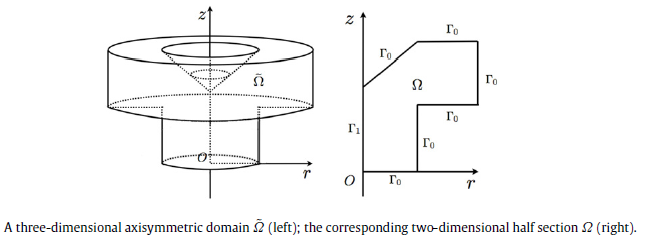
\includegraphics[width=1.0\textwidth]{projection_2D_general.PNG}
    \caption{Schematic projection on 2D half section}
    \label{projection_2D_general}
\end{figure}


- TODO: write this more formal
- Lax-Milgram-Lemma and Poincaré inequality on 3D-Domain determine a unique solution \\
- $u \in H^{1}_{r}(\Omega) \cap \{ v|_{\Gamma_{0}} \}  $
- Trace-operator \\
- rotation axis becomes an artificial boundary on 2D half section \\

- A more formal description can be found in : \\
- Use input from article TODO \\


\section{Discretization of PDEs}

\subsection{Computational Domain}
- Using one needle, whole geometry domain is axis symmetric around one needle \\
- Problem can be reduced to 2D problem using ring elements and cylindric coordinates \\
- Eliminate dependency on angular $\phi$ from the calculations \\
- For visualisation, symmetric results can be reconstructed to 3D \\
- Whole calculation will be in cylindric coordinates \\

\subsection{FEM in cylindric Coordinates}
- Rewrite the equations to cylindric coordinates \\
- Calculations are made on a cross-section with angular phi = 0 \\
- Define boundaries -> new artificial boundary around the rotation axis to be taken into consideration \\
- Explain how the new boundary can be treated \\
 
Laplace in cartesian coordinates:
\begin{equation}
    \nabla^2 := \Delta := \frac{\partial^2}{\partial x^2} + \frac{\partial^2}{\partial y^2} + \frac{\partial^2}{\partial z^2}
\end{equation}

Laplace in cylindric coordinates:
\begin{equation}
    \Delta := \frac{\partial^2}{\partial r^2} + \frac{1}{r} \frac{\partial}{\partial r} + \frac{1}{r^2} \frac{\partial^2}{\partial \phi^2} + \frac{\partial^2}{\partial z^2}
\end{equation}

TODO \\

Laplace in polar coordinates:
\begin{equation}
    \Delta := \frac{\partial^2}{\partial r^2} + \frac{1}{r} \frac{\partial}{\partial r} + \frac{1}{r^2} \frac{\partial^2}{\partial \phi^2}
\end{equation}



\subsection{PDE for Electric potential}

\subsubsection{Discretization of the problem}
4 areas can be distinguished from a mathematical point of view \\
- Inner domain \\
- Fixed Potential of electrodes \\
- Outer boundaries with no fixed potential -> Robin \\
- Rotation axis, artificial boundary -> Neumann \\

Constant material parameters -> \\
Coefficients are constants \\
This will simplify calculations and coupling \\

\subsubsection{Inner Domain}

- The electric potential of the inner domain is described as : 

\begin{equation}
    - \nabla \cdot (\sigma(x,y,z,t) \nabla \varphi(x,y,z,t)) = 0
\end{equation}

- Elliptical boundary problem \\
- Assuming constant material parameters: $\nabla \sigma = 0$ \\
- Solution is independent from $\sigma$ so we can cut it out
- Equation becomes Laplaces' equation, phi becomes time independent \\

\begin{equation}
    - \Delta \varphi(x,y,z) = 0
\end{equation}

- Using a cylindric domain, it is preferred to change coordinate systems \\
- Axis symmetry is given cylindrical coordinates (see ref Laplace in cylinder)

\begin{equation}
    - \Delta \varphi(r,\phi,z) = - \frac{1}{r} \frac{\partial \varphi}{\partial r} - \frac{\partial^2 \varphi}{\partial r^2} - \frac{1}{r^2} \frac{\partial^2 \varphi}{\partial \phi^2} -      \frac{\partial^2 \varphi}{\partial z^2}  = 0
\end{equation}

- Since the domain has axis symmetry, the solution for $\varphi$ is independent from the angular $\phi$ \\
- So equation basically simplifies to 

% \begin{equation}
  %  - \Delta \varphi(r,\phi,z) \overset{!}{=} - \Delta \varphi(r,z) = - \frac{1}{r} \frac{\partial %\varphi}{\partial r} - \frac{\partial^2 \varphi}{\partial r^2} - \frac{\partial^2 \varphi}{\partial %z^2} = 0
% \end{equation}

\begin{equation}
    - \nabla  ( \sigma \cdot \nabla \varphi(r,\phi,z)) \overset{!}{=} - \Delta \varphi(r,z) = - \frac{1}{r} \frac{\partial \varphi}{\partial r} - \frac{\partial^2 \varphi}{\partial r^2} - \frac{\partial^2 \varphi}{\partial z^2} = 0
\end{equation}

To keep the following descriptions simple, we will (ignore) "verzichten" the explicit dependencies r and z, since this is trivial

\subsubsection{Electrodes}

- Potential difference on the electrodes is fixed by definition \\
- For calculations, potential will be defined as $\pm 1$ chosen arbitrarily \\
- Bipolar probes have one fixed potential at each electrode

\begin{equation}
    \varphi = \pm 1
\end{equation}

- Other values would be possible too, but are rather unusual at monopolar probes \\

\subsubsection{Outer boundary}

- An easy approach is a simplification with natural boundary conditions \\

\begin{equation}
    n \cdot \nabla \varphi = 0
\end{equation}

- In cylindrical coordinates
\begin{equation}
    TODO
\end{equation}

- In actual RFA treatment, there is a mass to nullify the potential in the outer regions \\
- For the lower boundary, this behaviour can be easily modeled with dirichlet conditions \\
\begin{equation}
    \varphi = 0
\end{equation}

- Neither the neumann nor the dirichlet conditions actually reflect physics properly,, but is rather accurate enough for this approach \\
- Since there are made other simplifications, especially with the unrealistic "Annahme" of constant material parameters, this simplification of boundary conditions is within the margin ob acceptable errors


\subsubsection{Rotation axis}

- this is an artificial boundary, as discribed above \\
- To keep the axis symmetry, "leicht einsehbar" that here must natural boundary conditions \\
- Other conditions would break the trace operator \\
- A more mathematical description for this "Annahme" will described in the following chapter

- \begin{equation}
    n \cdot \nabla \varphi = 0
\end{equation}



\subsection{Calculation of electrical energy}

- $\varphi$ can be calculated on every discrete point \\
- Calculate power for every point with equations above (TODO add ref here) \\
- Phi is evaluated on discrete mesh points \\
- In a nutshell, Tissue Resistance and nonlinear behaviour of the generator generate an effective power which is as well the total power of the domain  a scalar multiplication factor for every discrete value for phi \\

- Thus leading to the calculation of the electric energy from electric power above \\


\subsection{PDE for temperature Distribution}

\subsubsection{Discretization of the problem}

From physics above, the temperature distribution is modeled by the heat equation: 

\begin{equation}
    \partial_t (\rho c T) - \nabla \cdot (\lambda \nabla T) = Q
\end{equation}

The heat equation is a well known parabolic partial differential equation. \\

T = T(r,z,t) = temperature \\
Q = Q(r,z,t) = heat energy \\

The material parameters are taken as constant, as described above \\
$\rho$ = density \\
$c$ = specific heat capacity, \\
$\lambda$ = thermal conductivity \\
- In temperature range of radio frequency ablation, $c$ and $\lambda$ are especially nonlinear depending on the temperature, for which the phase change of water is reason to \\ Evaporated water has a totally different heat capacity and thermal conductivty, also the transition is smooth and not abrupt \\


- However, Modeling the phase change of water and corresponding heat capacity does in practise lead to big numerical problems \\

- It is reasonable to at least model the temperature dependency of lambda, which leads to the following description

Cylindrical coordinates: see 'Transient Heat Transfer in a Partially Cooled Cylindrical Rod' from Lawrence Agbezuge

\begin{equation}
    \rho c \frac{\partial T}{\partial t} -  \frac{d\lambda}{dT} \left[ \left( \frac{\partial T}{\partial r} \right)^2 + \left( \frac{\partial T}{\partial z} \right)^2 \right] - \lambda \left( \frac{\partial^2 T}{\partial r^2} + \frac{1}{r} \frac{\partial T}{\partial r} + \frac{\partial^2 T}{\partial z^2} \right) = Q
\end{equation}

- For sake of simplicity in this academic approach, we will ignore the phase change of water willingly as a whole \\

- So it is "good" to assume that $lambda$ would also be constant too, which greatly reduces the complexity of the whole PDE \\

\begin{equation}
    \rho c \frac{\partial T}{\partial t} - \lambda \left( \frac{\partial^2 T}{\partial r^2} + \frac{1}{r} \frac{\partial T}{\partial r} + \frac{\partial^2 T}{\partial z^2} \right) = Q
\end{equation}

- The right hand side is described in the physics, see ref\\
- It is depending on the generated electrical energy and the cooling effect of perfusion \\

\begin{equation}
    Q_{total} = Q_{rf} + Q_{perf}
\end{equation}

- Since the material parameters are constant, $Q_{perf}$ can be easily evaluated linear depending on T for every discrete time step \\

\subsubsection{Needle}

- If we assume that the probe is cooled from outside, it is as simple and also accurate assumption to take the body temperature as constant temperature for the probe over the whole intervall
\begin{equation}
    T = T_{body} \
\end{equation}

- Usually body temperature is around $\cong$ 37 degree Celsius or 310.15 degree Kelvin \\
- If the probe is not cooled, another simple approach is to model the behaviour of needle likewise as the outer boundary \\  

\subsubsection{Outer boundary}

- Assuming there is no "Disturbing" from outside, natural boundary conditions conditions are the correct assumption for the heat equation  

- \begin{equation}
    n \cdot \nabla \varphi = 0
\end{equation}

- These can also be used to model non cooled probes \\

- In the following, we will discribe how the PDE models for $\varphi$ and $T$ can be transformed in the context of finite elements and numerically evaluated at discrete points \\


\section{Applied FEM technologies}

\subsection{Weak solutions}
\subsubsection{Electric potential}

Electric potential / Laplace's equation in cylindrical domain:

\begin{equation}
    a_w(u,v) := \int_{\Omega} (\partial_r u \partial_r v + \partial_z u \partial_z v) r drdz = \int_{\Omega} f v r dr dz
\end{equation}

\begin{align}
    u \in H_r^1(\Omega) \cap \{v|_{\Gamma_{0}} = 0 \} \\
    v \in H_r^1(\Omega) \cap \{v|_{\Gamma_{0}} = 0 \}     
\end{align}


Specific PDE for electric potential, inner domain: 

\begin{equation}
    a_w(u,v) := \int_{\Omega} (\partial_r u \partial_r v + \partial_z u \partial_z v) r drdz = 0 
\end{equation}

\subsubsection{Temperature Distribution}

This is basically the problem above but as a hyperbolic problem \\
Using semidiscrete solution and iterate solution over time \\
We are applying method of the discontinuous galerkein fem \\
For reference see Jung, Langer : Methode der finiten Elemente für Ingenieure, chapter 7.1 \\



Weak formulation for the problem: \\

We are looking for $u(r,z,t) \in V_{g1}$ with $\Dot{u} \in L_2(\Omega)$ for almost every $t \in (0,T)$, so \\ \begin{equation}
(\Dot{u},v)_0 + a(t;u,v) = \langle F(t),v \rangle \; for \; all \; v \in V_0    
\end{equation}
and for amost every $t \in (0, T)$ is the "Anfangsbedingung -> suche englische Formulierung"
\begin{equation}
    (u(r,z,0),v)_0 = (u_0,v)_0 \; for \; all \; v \in V_0
\end{equation}

The formal model above is given by 
\begin{align*}
    (\Dot{u},v)_0 &= \int_{\Omega} \Dot{u}(r,z,t)v(r,z) drdz = \int_{\Omega} \frac{\partial u(r,z,t)}{\partial t} v(r,z) drdz, \\
    a(t;u,v) &= \int_{\Omega} \left[ \lambda_1(r,z,t) \frac{\partial u}{\partial r} \frac{\partial v}{\partial r} + \lambda_2(r,z,t) \frac{\partial u}{\partial z} \frac{\partial v}{\partial z} \right] \cdot r \cdot drdz + \int_{\Gamma_3} \alpha(r,z,t)u(r,z,t)v(r,z) ds, \\
    \langle F(t),v \rangle &= \int_{\Omega} f(r,z,t)v(r,z) drdz + \int_{\Gamma_2} g_2(r,z,t)v(r,z) ds + \int_{\Gamma_3} \alpha(r,z,t)u_A(r,z,t)v(r,z) ds, \\
    V_{g_1} &= TODO, \\
    V_0 &= TODO
\end{align*}

Adapted for the temperature distribution, assuming $\lambda$ and all material parameters are constant: 

\begin{equation}
    a_w(t;u,v) := \int_{\Omega} \rho c (\partial_t u \cdot v) drdz + \int_{\Omega} \lambda (\partial_r u \partial_r v + \partial_z u \partial_z v) r drdz = \int_{\Omega} f v r dr dz
\end{equation}

\newpage


\subsection{Discretization / Triangulation}

- Grid generation and refinement \\
- 2D domain \\
- initial coarse grid trinagulation can be done by hand \\
- coarse grid can be refined by algorithm \\

- refinement of triangle into 4 new pieces \\
- \textcolor{blue}{insert picture here}

\subsection{Assembling system of equation}

- assemble elementwise \\
- Approximate elements with linear regression functions\\
- Calculation on reference triangles to speed up performance and accuracy \\

Linear regression functions for reference triangles:
\begin{align}
    \phi_1(\xi, \eta) &= 1 - \xi - \eta \\
    \phi_2(\xi, \eta) &= \xi \\
    \phi_2(\xi, \eta) &= \eta 
\end{align}

- use symmetrie of elements if coefficients are constant or allow it \\
- Add boundary conditions afterwards \\
- grouping of similar calculations allow more vectorized operations \\ 

\subsection{ODE for parabolic problems}

\textcolor{blue}{TODO}

\subsection{Solving the system of equations}
- direct solver would be preferred in general \\
- if numbers of element grows, this computations takes up lots of memory \\
- up from a certain point, high amount memory can't be efficiently handled with RAM anymore \\
- using additional memory is extremely costly in terms of calculation speed \\
- since matrix is sparse, iterative solver can be very fast \\
- iterative solver is preferred if elements grow in numbers \\
- TODO : when should you use iterative solver \\

\subsection{Error estimations}

\subsubsection{Element Error on 2D geometry}
- H1-Norm \\
- L2-Norm \\

- The analytical solution of the problem is unknown, but we can estimate it by calculating different element sizes on different sized fine grids \\

Idea: Define geometric some geometric coordinates on triangle and look for best matching or choose some points on different geometrical entities \\

Refine triangles around that point and see whether the error is smaller on the finer grid \\

\subsubsection{Time step error on discrete intervalls}

See Skript Numerik 2 Kroeger, after some take make a smaller or larger time step and compare the difference of results, use the smaller steps for calculation \\


\newpage


\section{Other numerical aspects }


\subsection{Surface integral}
- Sum of integral of every single triangle \\
- Single triangle on discrete gauss quadrature points \\
- Can use more nodes, which is usually worth the calculation effort \\
- Implemented on 3 or 7 points \\
- TODO insert picture \\

\subsection{Numerical gradient on discrete points}
- Trial functions approach the solution of the variation problem \\
- in our case, gradient is constant on every triangle \\
- actually discrete gradient on vertices is interesting \\
- vertices as average value of surrounding the sorrounding triangles \\

\subsection{Grid refinement}
- Refine triangle uniformly into 4 new ones \\
- Can be done as efficient vector operation \\

\subsection{Troublesome neighbours}
- Collision on corner nodes and boundaries of electrodes \\
- Corner node is defined well for dirichlet as well as for neumann conditions \\
- Handling dirichlet nodes is done by setting row and column vectores to zero and rhs to dirichlet value, which is a problem for the neumann boundary  \\
- Dirichlet value has higher priority for corners \\
- This is a problem for the node on the neumann boundary next to the corner \\
- So this exactly neumann node has some unforseen behaviour \\
- To handle this, best way has shown to be to ignore the result for this node and interpolate the result by weighing the neighboring nodes \\  
- This particular solution might have its obvious flaws, but gets pretty good results in practise \\


\section{Applied simulation}
\subsection{Generating TestData / Get reference data}
- Material parameters see Stein TODO \\
- Using specification data from electrical generator TODO \\

\subsection{Solving the PDEs}

\subsection{Combine everything to continous time dependent simulation}

\subsection{Interpretation of result numbers}
- Interprete numbers \\
- Compare with data from experiment or other simulations \\
- TODO compare with other simulations \\

\section{Programming technologies}

\subsection{Performance Optimization}
\subsection{MatLab vs C++}
- Could have done the whole simulation using only MATLAB \\
- MATLAB is a scripting language that calls Fortran Subroutines, which are highly efficient in calculating problems of linear algebra \\
- However, MATLAB has to call these subroutines in an efficient way to take these performance advantages \\
- It is extremely easy to write bad and inperformant code in MATLAB, if it is used in the wrong way \\
- Efficient implementation required hardcoding routines and is very stiff \\ 
- To me it was important to write flexible code, that can be easily adapted and extended to try out different modification \\
- This is way easier when using loops and subroutines instead of hard coded implementations, also the code because way more easier to read and fix \\
- So I was going for a combined implementation of MatLab and C++ \\ 
- When using flexible code design, C++ allows performance advantages in using loops etc over MATLAB \\
- However, MATLAB allows easy function hadnling, what makes the algorithms more accessable for the reader \\ 
- In the end I combined the advantages of both languages \\
- MatLab serves as frame for the pre- and postprocessing, like grid generation and graphical output of the numerical results. \\
- Also the scripts serve as a mathematical documentation of the whole simulation for the reader \\
- Computation intense subroutines are done in C++ \\


\subsection{Graphical output}
- Data can be easily recreated \\
- Solution is axis symmetric, so values apply for every angle $\phi$ \\
- This gets 3D data in cylindrical coordinates \\
- Can be reevaluated into cartesian coordinates to be plotted \\
- Discrete points are linear interpolated \\


% part 3, Summary

\section{Summary and Outlook}

\subsection{Project Summary}
- One could argue that writing a numerical simulation from scratch is a waste of time \\
- There are many highly useful numerical software solutions for numerical simulation and numerical problems \\
- Usually there is no need to write an own detailed implementation \\
- However, creating own scripts and implementations helps to understand numerical problems and error sources \\
- This approach helps enormously to increase the ability to use these software products effectively and to generate better simulations and is mandatory to improve \\
- There can also be no software developer without understanding how a computer works numbers \\
- Implementing the algorithms on own trains understanding of numerical problems \\
- Should be programmed by everyone working with finite elements at least once \\

\subsubsection{strengths and flaws}
- good: numerical results do match the general expectation \\
- "zuverlässige" convergency \\
- numerical solution matches "qualitativ" the expectations \\
- Implementation can be easily adopted to more complex approaches \\

- bad: model is way to simplified to represent real world conditions of RFA \\
- Even further modifications would not change the results heavily \\

\subsubsection{future modifications}
- Material parameters are dependent on Temperature and potential -> \\
- Using variable instead of fixed material parameters \\
- Take the evaporation of water into account \\ 
- Different types of perfusion \\
- Defining more realistic and complex boundary conditions \\
- Perhaps a second needle in a 3D simulation \\
- Basic algorithm can be adopted to 3D problems \\

\subsection{State of the current Research}
- Research in the simulation of medical therapy methods \\
- TODO \\


\subsection{Other FEM projects and software}

- There is a lot of good commercial FEM software out there \\
- Matlab PDE toolbox, libraries with efficient implementation of almost every aspect on solving PDEs \\
- COMSOL Multiphysics, a High-Power simulation program with model builder and GUI \\
- ANSYS, like COMSOL but a little weaker but more widely used\\

- Also, good open source software \\
- FENICS \\
- FREEFEM \\


\newpage


%% Literature register using .bib file
\clearpage
\nocite{*}
\printbibliography

\newpage

%% last part, appendix
\appendix

%!TeX root=Main.tex

% Dieses File ist für den Anhang
% Hier kann potenzieller Quellcode generiert werden
% Sowie zusätzliche Bilder usw eingefügt werden
% Wird nicht für alle Versuche benötigt werden

\section{Source code Visual C++}

\lstset{language=C++,
                basicstyle=\ttfamily,
                keywordstyle=\color{blue}\ttfamily,
                stringstyle=\color{red}\ttfamily,
                commentstyle=\color{gray}\ttfamily,
                morecomment=[l][\color{orange}]{\#}
}

\begin{lstlisting}[caption={[Demo] For loop to print numbers from 1 to 10}]
// Print numbers from 1 to 10
#include <stdio.h>
int main() {
  int i;
  for (i = 1; i < 11; ++i)
  {
    printf("%d ", i);
  }
  return 0;
}
\end{lstlisting}


\section{Source code MatLab}

\Large{TODO}
 

\end{document} 